\documentclass[aspectratio=169]{beamer}
\usetheme[numbering=fraction]{metropolis}

% TikZ packages
\usepackage{tikz}
\usetikzlibrary{arrows.meta, positioning}

% TikZ styles
\tikzset{
    block/.style={
        rectangle,
        draw,
        rounded corners=2pt,
        minimum width=6em,
        minimum height=2.5em,
        align=center
    },
    arrow/.style={
        -{Latex},
        thick
    }
}

\begin{document}

% -------------------- Slide 1 --------------------
\begin{frame}{MQTT Protocol}
\begin{itemize}
    \item Lightweight messaging protocol for IoT.
    \item Based on publish/subscribe architecture.
    \item Enables real-time monitoring of:
    \begin{itemize}
        \item Temperature
        \item Humidity
        \item Light Levels
        \item Air Quality
    \end{itemize}
    \item Ensures efficient communication between devices and apps.
\end{itemize}
\end{frame}

% -------------------- Slide 2 --------------------
\begin{frame}{System Block Diagram}
\centering
\vspace{0.75cm}
\resizebox{1.0\textwidth}{0.8\textheight}{% scale to fit slide
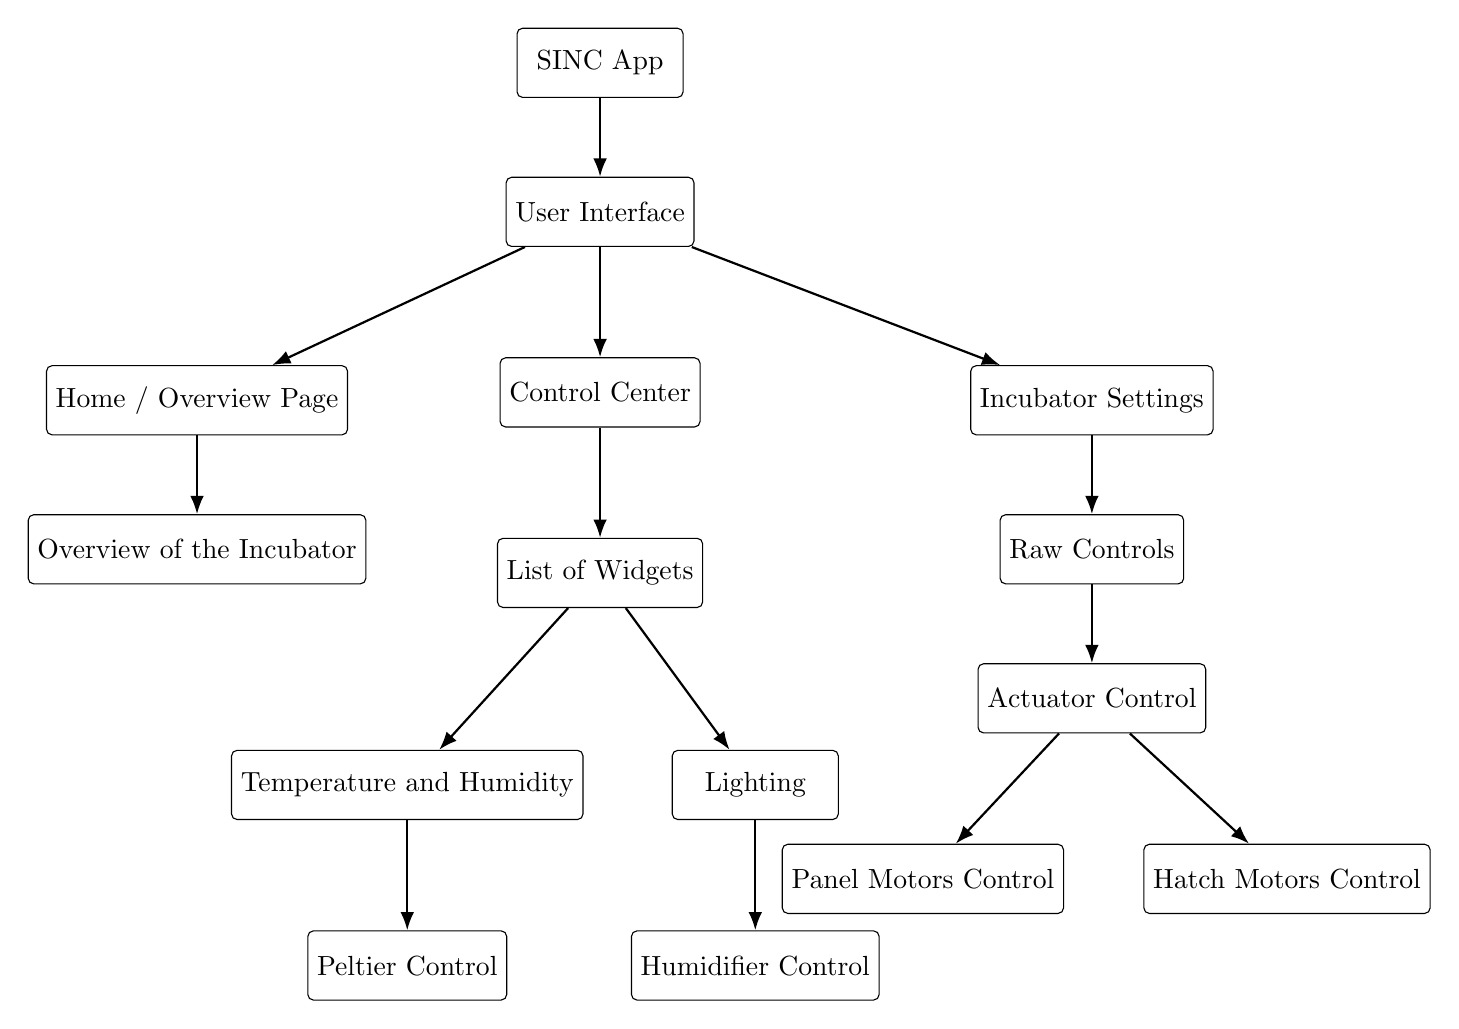
\begin{tikzpicture}[node distance=1.4cm and 2cm]

% Top Layer
\node[block] (app) {SINC App};
\node[block, below=1.0cm of app] (ui) {User Interface};

% Second Layer
\node[block, below left=1.5cm and 2.0cm of ui] (home) {Home / Overview Page};
\node[block, below=of ui] (controlcenter) {Control Center};
\node[block, below right=1.5cm and 3.5cm of ui] (incsettings) {Incubator Settings};

% Third Layer
\node[block, below=1.0cm of home] (overview) {Overview of the Incubator};
\node[block, below=of controlcenter] (widgets) {List of Widgets};
\node[block, below=1.0cm of incsettings] (rawcontrols) {Raw Controls};

% Fourth Layer
\node[block, below left=1.8cm and -1.1cm of widgets] (temphum) {Temperature and Humidity};
\node[block, below right=1.8cm and -0.4cm of widgets] (lighting) {Lighting};
\node[block, below=1.0cm of rawcontrols] (actuator) {Actuator Control};

% Fifth Layer
\node[block, below=of temphum] (peltier) {Peltier Control};
\node[block, below=of lighting] (humidifier) {Humidifier Control};
\node[block, below left=1.4cm and -1.1cm of actuator] (panelmotors) {Panel Motors Control};
\node[block, below right=1.4cm and -0.8cm of actuator] (hatchmotors) {Hatch Motors Control};

% Connections
\draw[arrow] (app) -- (ui);
\draw[arrow] (ui) -- (home);
\draw[arrow] (ui) -- (controlcenter);
\draw[arrow] (ui) -- (incsettings);

\draw[arrow] (home) -- (overview);
\draw[arrow] (controlcenter) -- (widgets);
\draw[arrow] (incsettings) -- (rawcontrols);

\draw[arrow] (widgets) -- (temphum);
\draw[arrow] (widgets) -- (lighting);
\draw[arrow] (rawcontrols) -- (actuator);

\draw[arrow] (temphum) -- (peltier);
\draw[arrow] (lighting) -- (humidifier);
\draw[arrow] (actuator) -- (panelmotors);
\draw[arrow] (actuator) -- (hatchmotors);

\end{tikzpicture}
} % end resizebox
\end{frame}

% -------------------- Slide 3 --------------------
\begin{frame}{Future Enhancements}
\begin{itemize}
    \item Integration with real IoT sensors for live monitoring.
    \item Cloud-based storage and analytics.
    \item AI-driven predictions for optimized control.
    \item Scalable design for advanced smart environments.
\end{itemize}
\end{frame}

% -------------------- Slide 4 --------------------
\begin{frame}{App UI Overview}
\centering
\begin{tabular}{cccc}
\vspace{0.5cm}
    \includegraphics[width=0.22\textwidth]{app4.jpeg} &
    \includegraphics[width=0.22\textwidth]{app5.jpeg} &
    \includegraphics[width=0.22\textwidth]{app2.jpeg}&
    \includegraphics[width=0.22\textwidth]{app6.jpeg}\\
    \textbf{Home} & \textbf{Status} & \textbf{Settings} &\textbf{Alerts}\\
\end{tabular}
\end{frame}

\end{document}
